\section*{Выполнение задания}
Изначально был изменён параметр SystemID в QSYS. 
Мой вариант -- 6, группа -- 55.

Результат представлен на рисунке 7.

\FloatBarrier
\begin{figure}[h]
	\begin{center}
		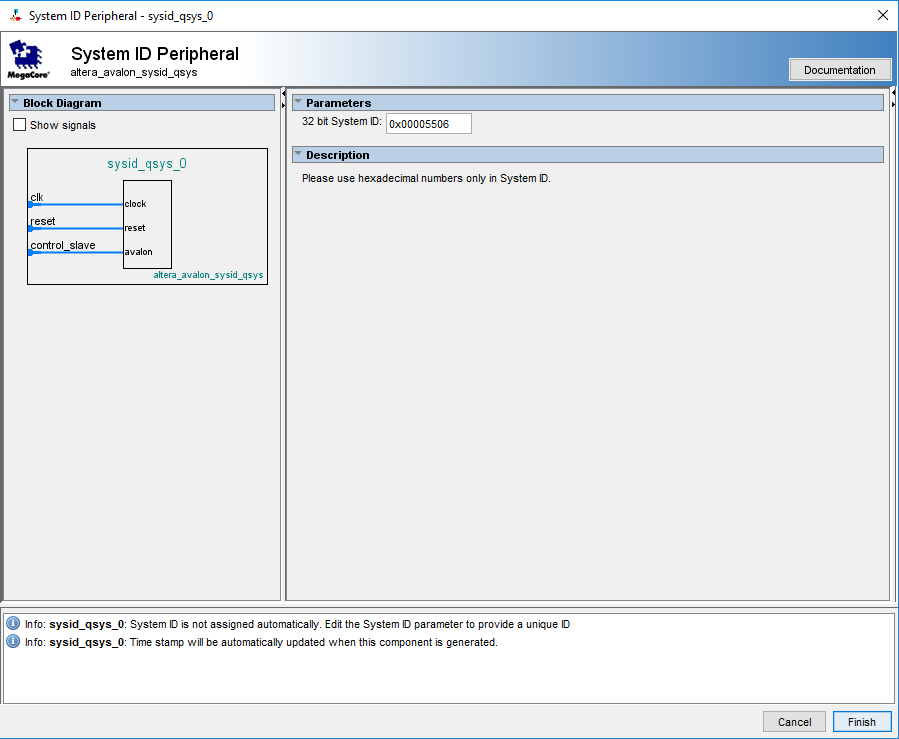
\includegraphics[width=\linewidth]{inc/newID.png}
	\end{center}
	\caption{Назначение параметра SystemID в соответствии с вариантом}
\end{figure}
\FloatBarrier

Затем к ПК была подключена отладочная плата с ПЛИС ЕРС2С20.
Была выполнена верификация проекта с использованием программы терминала.

Параметры для терминала представлены на рисунке 8.
\FloatBarrier
\begin{figure}[h]
	\begin{center}
		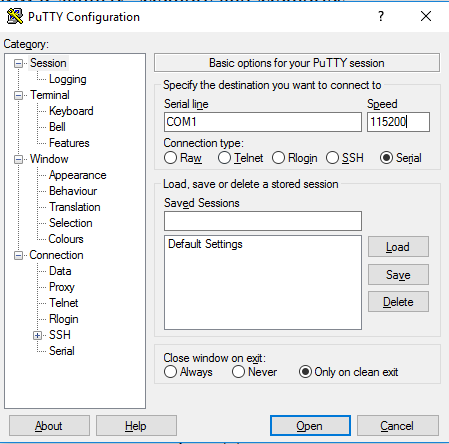
\includegraphics[width=\linewidth]{inc/command.png}
	\end{center}
	\caption{Параметры для терминала}
\end{figure}
\FloatBarrier

Итоговый вывод представлен на рисунке 9.
\FloatBarrier
\begin{figure}[h]
	\begin{center}
		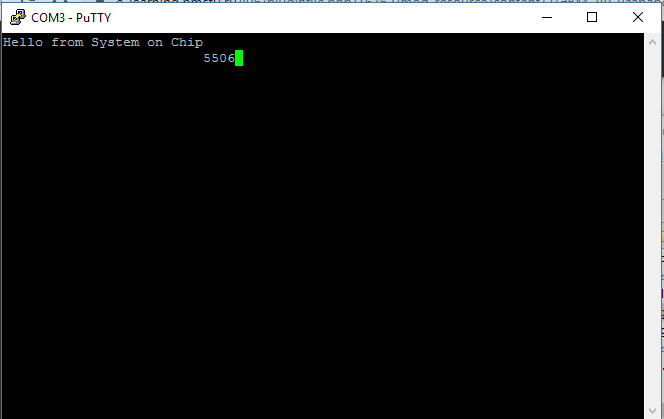
\includegraphics[width=\linewidth]{inc/result.png}
	\end{center}
	\caption{Итоговый вывод}
\end{figure}
\FloatBarrier